 \documentclass[fontsize=8pt,paper=A4, DIV=9]{scrartcl}

\usepackage{fancyhdr}
 \usepackage[utf8]{inputenc}
% \usepackage[T1]{fontenc}
\usepackage{enumerate} 
 %\usepackage{lmodern}
 \usepackage{amsmath}
 %\usepackage{amssymb}
 \usepackage{relsize}
 \usepackage{xparse}
%\documentclass{book}
\usepackage{color}
\usepackage{float}
%\usepackage{amsmath}
%]{standalone}
\makeatletter
\let\@oddfoot\@empty
\let\@evenfoot\@empty
\makeatother
\usepackage{tikz}
\usetikzlibrary{automata,positioning, arrows}
\usetikzlibrary{patterns, arrows}
\usetikzlibrary{arrows.meta,shapes.arrows}
%\usetikzlibrary{decorations.markings}
\tikzset{->, % makes the edges directed
>=stealth, % makes the arrow heads bold
node distance=2.4cm, % specifies the minimum distance between two nodes. Change if necessary.
every state/.style={thick, fill=gray!10}, % sets the properties for each ’state’ node
initial text=$ $, % sets the text that appears on the start arrow
}
%\fancyhead{}
%\fancyhead[RO]{Turing Machine  }
%\fancyhead[LE]{ Introduction to Automata Theory, Formal Languages and Computation}
%\fancyhead[LE,RO]{$\thepage$}
%\fancyfoot{}

%\renewcommand{\headrulewidth}{}

%\pagestyle{fancy}
%%%%%%%%%%%%%%%%%%%%%%%%%%%% The paper headers
%\fancyhead[RO,LE]{\small\thepage}
%\fancyhead[LO]{\small Turing Machine}% odd page header and number to right top
%\fancyhead[RE]{\small Introduction to Automata Theory, Formal Languages and Computation}%Even page header and number at left top
%\fancyfoot[L,R,C]{}%-----------
%\renewcommand{\headrulewidth}{0pt}% disable the underline of the header part

%-------------------------

%----------------------------
\begin{document}
%\thispagestyle{plain}
\vspace*{-3.5cm}
%\begin{center}
%\includegraphics[height=2.2cm, width=18cm]{headerpic}
%\end{center}
%\vspace*{0.5cm}

\begin{flushright}
 Turing$ $ Machine $| $445
\end{flushright}

%\vspace*{0.5cm}

%{\small First Author}\index{Familyname, Name}\footnote{speaker}\\
%{\small Faculty of ..., University of...}\\[2mm]
%{\small Second Author}\index{Family Name, Name}\\
%{\small  Faculty of ..., University of...}\\[2mm]
%{\small Third Author}\index{Family Name, Name}\\
%{\small  Faculty of ..., University of...}\\[2mm]


\vspace*{0.5cm}

%\hspace{-1cm}\rule{\textwidth}{0.2mm}
%%%%%%%%%%%%% abstract %%%%%%%%%%%%%

%\keywords{At most 5 words or phrases.}
%\subject{Primary: 22D15, 43A10; Secondary: 43A20, 46H25}

%\hspace{-1cm}\rule{\textwidth}{0.2mm}

%----------------------------------------------------------------------
%----------------------------------------------------------------------
%----------------------------------------------------------------------
\section*{8.2 Transitional Representation of Turing Machine}
%----------------------------------------------------------------------
%----------------------------------------------------------------------
%----------------------------------------------------------------------
The mathematical notation for a TM is $(Q, \Sigma,\Gamma,\sigma, q0
, B, F)$. In a TM, the transitional function $\sigma$ consists
of the form $ Q \times \Gamma \rightarrow (Q  \times \Gamma  \times \lbrace L, R, H \rbrace)$, where the first is a present state and the second is the present
input (single character $\in \Gamma$ ). The transition produces a state, a symbol $\in \Gamma$ written on the input tape, and
the head moves either left or right or halts.

In the graphical notation of the TM, there are states. Among them, a circle with an arrow indicates a
beginning state and a state with double circle indicates a final state, where the machine halts finally. The state
transitions are denoted by arrows. The labels of the state transitions consist of the input symbol, the symbol
written on the tape after traversal, and the direction of movement of the read–write head (left, right, or halt).
The following are some examples of the TM with the transitional representation.

% 

%\begin{frame}

%\tikz\node at (2,0) [fill=black,shape=single arrow,text width=2cm,text height=0.5cm ] {};


%\end{frame}


    %------------------------
    \begin{figure}[H] % ’ht’ tells LaTeX to place the figure ’here’ or at the top of the page
%\centering % centers the figure
 
\begin{tikzpicture}[every node/.style={single arrow, draw=none, }]

        \node [fill=black,text=white, single arrow head indent=1ex] at (-1.5,0) {Example 8.16};
    \end{tikzpicture}
   Design a TM by the transitional notation for the language $L = a^{n}
b^{n}$, where $ n > 0$.
\end{figure}
    %------------------------
\textbf{Solution:} When the machine traverses ‘a’, replace that ‘a’ by X and traverse right to find the leftmost
‘b’. Replace that ‘b’ by ‘Y’ and traverse left to find the second ‘a’. The second ‘a’ exists after ‘X’, which
was replaced first for the fi rst ‘a’. By this process, when n number of ‘a’ and n number of ‘b’ are traversed and replaced by X and Y, respectively, then by getting a blank (B) the machine halts.
The transitional representation of the TM is given in Fig. 8.2 .

\begin{figure}[H] % ’ht’ tells LaTeX to place the figure ’here’ or at the top of the page
\centering % centers the figure
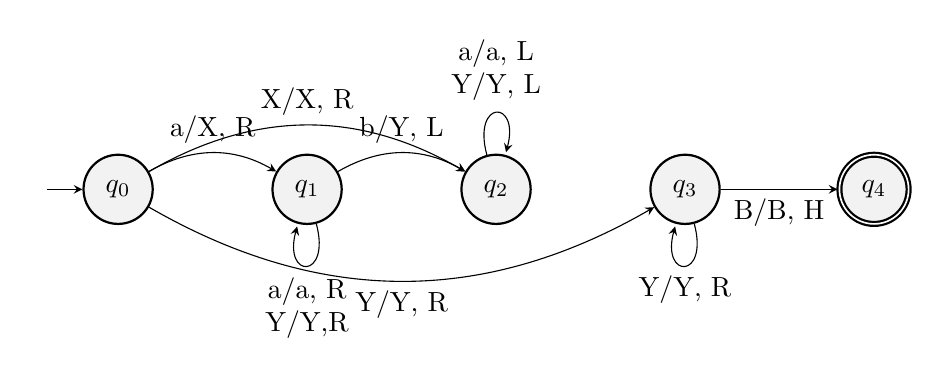
\begin{tikzpicture}
\node[state, initial] (q0) {$q_0$};
\node[state, right of=q0] (q1) {$q_1$};
\node[state, right of=q1] (q2) {$q_2$};
\node[state, right of=q2] (q3) {$q_3$};
\node[state, accepting, right of=q3] (q4) {$q_4$};


\draw 
(q0) edge[bend left,above] node{a/X, R} (q1)
(q1) edge[loop below] node{\begin{tabular}{c} a/a, R \\ Y/Y,R  \end{tabular}
 } (q1)

(q1) edge[bend left,above] node{b/Y, L} (q2)

(q2) edge[loop above] node{\begin{tabular}{c} a/a, L \\ Y/Y, L  \end{tabular}
} (q2)
(q0) edge[bend left,above] node{X/X, R} (q2)
(q0) edge[bend right, below] node{Y/Y, R} (q3)
(q3) edge[loop below,below] node{Y/Y, R} (q3)
(q3) edge[above,below] node{B/B, H} (q4);


\end{tikzpicture}
%\caption*{Caption.}


 \textbf{Fig. 8.2}\textit{ Transitional Representation of Turing Machine}
\label{ Fig. 8.2}
\end{figure}
\begin{figure}[H] % ’ht’ tells LaTeX to place the figure ’here’ or at the top of the page
%\centering % centers the figure
 
\begin{tikzpicture}[every node/.style={single arrow, draw=none, }]

        \node [fill=black,text=white, single arrow head indent=1ex] at (-1.5,0) {Example 8.17};
    \end{tikzpicture}
   Design a TM by transitional notation for the language L =$\lbrace $set of all palindrome over a,b$\rbrace$.
\end{figure}
\textbf{Solution:} A palindrome can be of two types, namely, an odd palindrome and an even palindrome. A null
string is also a palindrome. There are three paths to reach to the final state with halt from q1
, the beginning state. This is described in Fig. 8.3.
\begin{figure}[H] % ’ht’ tells LaTeX to place the figure ’here’ or at the top of the page
\centering % centers the figure
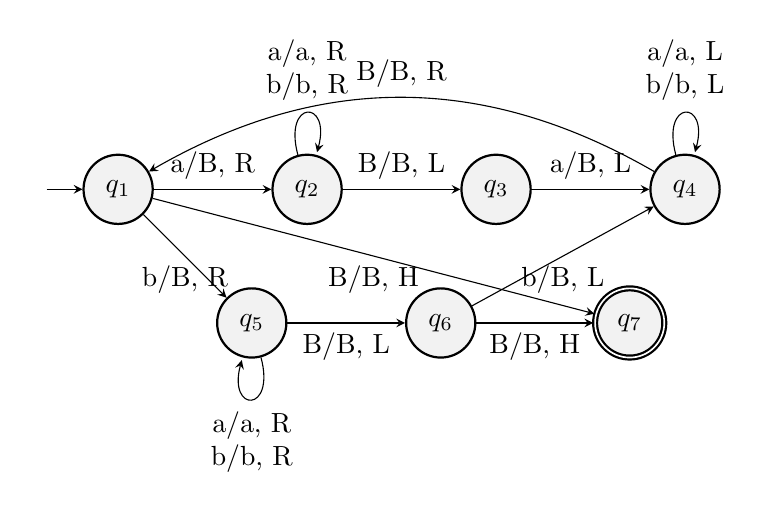
\begin{tikzpicture}
\node[state, initial] (q1) {$q_1$};

\node[state, right of=q1] (q2) {$q_2$};
\node[state, right of=q2] (q3) {$q_3$};
\node[state, right of=q3] (q4) {$q_4$};
\node[state, below right of=q1 ] (q5) {$q_5$};
\node[state, right of=q5] (q6) {$q_6$};

\node[state, accepting, right of=q6] (q7) {$q_7$};
\draw 



(q1) edge[left,above] node{a/B, R} (q2)

(q2) edge[loop above] node{\begin{tabular}{c} a/a, R \\ b/b, R  \end{tabular}
} (q2)
(q2) edge[left,above] node{B/B, L} (q3)
(q3) edge[left,above] node{a/B, L} (q4)
(q4) edge[loop above] node{
\begin{tabular}{c} a/a, L \\ b/b, L  \end{tabular}
} (q4)
(q4) edge[bend right,above] node{B/B, R} (q1)
(q1) edge[left, below] node{b/B, R} (q5)
(q1) edge[left, below] node{B/B, H} (q7)
(q5) edge[loop below] node{\begin{tabular}{c} a/a, R \\ b/b, R  \end{tabular}
} (q5)
(q6) edge[left, below] node{b/B, L} (q4)
(q5) edge[left, below] node{B/B, L} (q6)

(q6) edge[above,below] node{B/B, H} (q7);



\end{tikzpicture}


 \textbf{Fig. 8.3}\textit{Turing Machine for Set of All Palindrome Over a, b} 
\label{ Fig. 8.3}
\end{figure}
 

\pagebreak 

\vspace*{-3.5cm}
\begin{flushleft}
446 $ | $ Introduction$ $ to$ $ Automata$ $ Theory,$ $ Formal$ $ Languages$ $ and$ $ Computation
\end{flushleft}
\vspace*{0.5cm}

%-------------------------------------------
%---------------------------------------------------------------------------------
\section*{8.3  Non-deterministic Turing Machine}
The concept of non-determinism is clear as we have already discussed about NDFA or NDPDA in the
earlier chapters. There is also a non-deterministic TM. A non-deterministic TM is defi ned as $(Q,\Sigma,\Gamma, \sigma,
q0
, B, F)$, where $\sigma$ is $Q \times\Gamma\rightarrow 2^{Q X }  \Gamma^{X  \lbrace L,R \rbrace}$.


Let there exist a transitional function $\sigma(q0
, 0)\rightarrow (q0
, 0, R), (q1
, 1, R)$.

For traversing the input symbol, we have to consider two transitions and construct the following
transitions accordingly.
The NTM is more powerful than the DTM. An NTM $T_{1}$
 can be simulated to an equivalent DTM $T_{2}$.
One of the methods is to construct a computation tree of the NTM and perform a breadth first search of
the computation tree from the root until the halt state is reached. At each level of the constructed tree, $T_{2}$
uses the transitional functions of $T_{1}$
 to each confi guration at that level and computes its children. These
children are stored on a tape for the confi guration of the next level. Among the children, if the halting
state exists then $T_{2}$
 halts by accepting the strings. $T_{2}$
 accepts means that one branch of $T_{1}$
 accepts it. It
can be said that $T_{2}$
 accepts a string if and only if $T_{1}$
 accepts it.
 
 Any language accepted by an NTM is also accepted by a DTM. But the time taken by a DTM to
accept a language is more than the time taken by an NTM. In most of the cases, it is exponential in
length. A famous unsolved problem in computer science, i.e., the P = NP problem, is related to this issue.


 \begin{figure}[H] % ’ht’ tells LaTeX to place the figure ’here’ or at the top of the page
%\centering % centers the figure
 
\begin{tikzpicture}[every node/.style={single arrow, draw=none, }]

        \node [fill=black,text=white, single arrow head indent=1ex] at (-1.5,0) {Example 8.18};
    \end{tikzpicture}
  Construct a TM over $\lbrace a, b \rbrace$ which contains a substring abb.
\end{figure}

Solution: In regular expression, it can be written as $(a, b)^{*}
abb(a, b)^{*}$
. In this expression, the substring
is important. The string may be abb only. In that case, the machine gets ‘a’ as input in the beginning
state. Before traversing the substring ‘abb’, there is a chance to traverse ‘a’ of $\lbrace a, b\rbrace^{*}$
. The transitional functions are
\begin{center}
$\sigma(q1, a) \rightarrow (q1, a, R), (q2, a, R)$


$\sigma(q1, b) \rightarrow (q1, b, R)$


$\sigma(q2, b) \rightarrow (q3, b, R)$


$\sigma(q3, b)  \rightarrow (q4, b, R)$


$\sigma(q4, a)  \rightarrow (q4, a, R)$


$\sigma(q4, b) \rightarrow (q4, b, R)$


 $\sigma(q4, B) \rightarrow (qf , B, H)$
\end{center}

In state $q_{1}$
 for input ‘a’, there are two transitional functions. So, it is a non-deterministic TM.
%----------------------------------------------------------------------

%----------------------------------------------------------------------
\section*{8.4 Conversion of Regular Expression to Turing Machine}

Regular expression can be converted to an equivalent TM. The process is as follows.
 \begin{enumerate}
 \item  Convert the regular expression to an equivalent automata without the $\in$ move.
 \item  Change both the initial and fi nal states of the automata to an intermediate state.
 \item  Insert a new initial state with a transition (B, B, R) to the automata’s initial state.
 \item   Convert the transitions with label ‘ip’ to (ip, ip, R).
 \item  5. Insert a new fi nal state with a transition (B, B, R) from the automata’s fi nal state to the new
fi nal state.
 \end{enumerate}
 
 %----------------------------------------------------------------------
%----------------------------------------------------------------------
\pagebreak
\vspace*{-3.5cm} 
\begin{flushright}
 Turing$ $ Machine $| $447
\end{flushright}
\vspace*{0.5cm}
%------------------------------------------------
 \begin{figure}[H] % ’ht’ tells LaTeX to place the figure ’here’ or at the top of the page
%\centering % centers the figure
 
\begin{tikzpicture}[every node/.style={single arrow, draw=none, }]

        \node [fill=black,text=white, single arrow head indent=1ex] at (-1.5,0) {Example 8.19};
    \end{tikzpicture}
  Construct a TM for the regular expression $(a + b)^{*}(aa + bb)(a + b^{*})$.

\end{figure}
\textbf{Solution:} The finite automata accepting the regular expression is
\begin{figure}[H] % ’ht’ tells LaTeX to place the figure ’here’ or at the top of the page
\centering % centers the figure
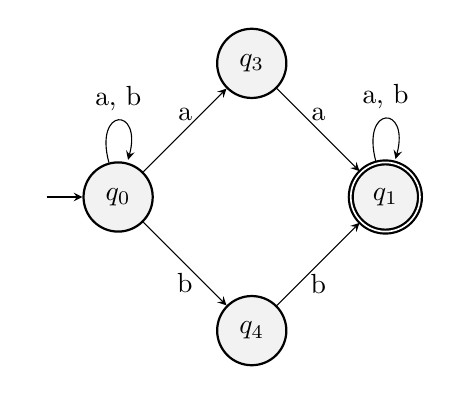
\begin{tikzpicture}
\node[state, initial] (q0) {$q_0$};
\node[state,above right of=q0] (q3) {$q_3$};

\node[state,  below right of=q0] (q4) {$q_4$};
\node[state, accepting, below right of=q3] (q1) {$q_1$};


\draw 

(q0) edge[loop above] node{a, b } (q0)
(q0) edge[left,above] node{a} (q3)
(q0) edge[left,below] node{b} (q4)
(q3) edge[left,above] node{a} (q1)
(q4) edge[left,below] node{b} (q1)
(q1) edge[loop above] node{a, b } (q1);


\end{tikzpicture}
%\caption*{Caption.}

\end{figure}

Inserting a new initial state $q_{i}$
 and final state $q_{H}$, the fi nite automata becomes
%----------------------------------------------------------------------
%----------------------------------------------------------------------
\begin{figure}[H] % ’ht’ tells LaTeX to place the figure ’here’ or at the top of the page
\centering % centers the figure
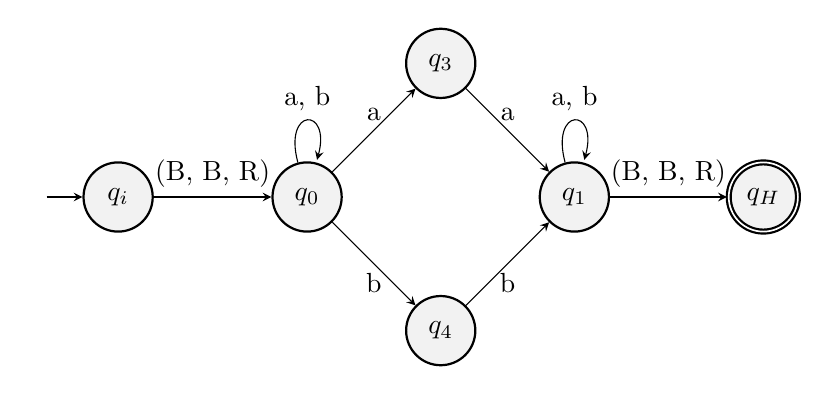
\begin{tikzpicture}
\node[state, initial] (qi) {$q_i$};
\node[state, right of=qi] (q0) {$q_0$};
\node[state,above right of=q0] (q3) {$q_3$};

\node[state,  below right of=q0] (q4) {$q_4$};
\node[state, below right of=q3] (q1) {$q_1$};
\node[state, accepting, right of=q1] (qH) {$q_H$};


\draw 
(qi) edge[right, above] node{(B, B, R) } (q0)
(q0) edge[loop above] node{a, b } (q0)
(q0) edge[right,above] node{a} (q3)
(q0) edge[right,below] node{b} (q4)
(q3) edge[right,above] node{a} (q1)
(q4) edge[right,below] node{b} (q1)
(q1) edge[loop above] node{a, b } (q1)
(q1) edge[right, above] node{(B, B, R) } (qH);

\end{tikzpicture}
%\caption*{Caption.}

\end{figure}

Converting the levels of the inputs, the TM becomes
\begin{figure}[H] % ’ht’ tells LaTeX to place the figure ’here’ or at the top of the page
\centering % centers the figure
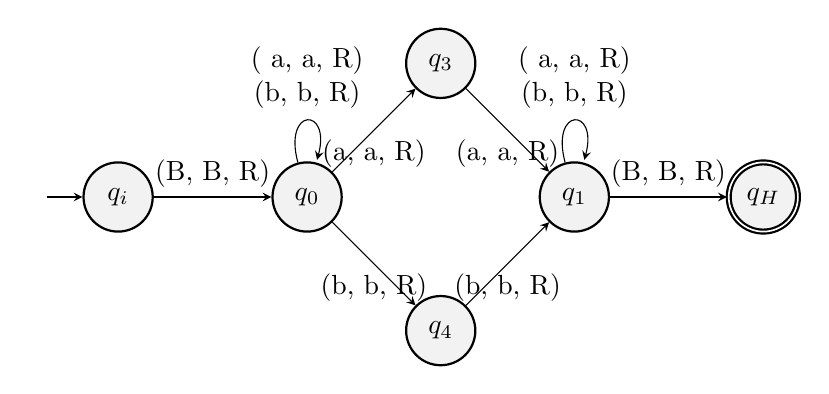
\begin{tikzpicture}
\node[state, initial] (qi) {$q_i$};
\node[state, right of=qi] (q0) {$q_0$};
\node[state,above right of=q0] (q3) {$q_3$};

\node[state,  below right of=q0] (q4) {$q_4$};
\node[state, below right of=q3] (q1) {$q_1$};
\node[state, accepting, right of=q1] (qH) {$q_H$};


\draw 
(qi) edge[right, above] node{(B, B, R) } (q0)
(q0) edge[loop above] node{\begin{tabular}{c} ( a, a, R) \\ (b, b, R)  \end{tabular}  } (q0)
(q0) edge[right,below] node{(a, a, R)} (q3)
(q0) edge[right,below] node{(b, b, R)} (q4)
(q3) edge[right,below] node{(a, a, R)} (q1)
(q4) edge[right,below] node{(b, b, R)} (q1)
(q1) edge[loop above] node{\begin{tabular}{c} ( a, a, R) \\ (b, b, R)  \end{tabular}} (q1)
(q1) edge[right, above] node{(B, B, R) } (qH);

\end{tikzpicture}
\end{figure}

\pagebreak 

\vspace*{-3.5cm}
%------------------------------------------
\begin{flushleft}
448 $ | $ Introduction$ $ to$ $ Automata$ $ Theory,$ $ Formal$ $ Languages$ $ and$ $ Computation
\end{flushleft}
\vspace*{0.5cm}


%---------------------------------------------

 \begin{figure}[H] % ’ht’ tells LaTeX to place the figure ’here’ or at the top of the page
%\centering % centers the figure
 
\begin{tikzpicture}[every node/.style={single arrow, draw=none, }]

        \node [fill=black,text=white, single arrow head indent=1ex] at (-1.5,0) {Example 8.20};
    \end{tikzpicture}
 Construct a TM for the regular expression $ab(aa + bb)(a + b)^{*}b$.

\end{figure}

\textbf{Solution:} The finite automata accepting the regular expression is

%----------------------------------------
\begin{figure}[H] % ’ht’ tells LaTeX to place the figure ’here’ or at the top of the page
\centering % centers the figure
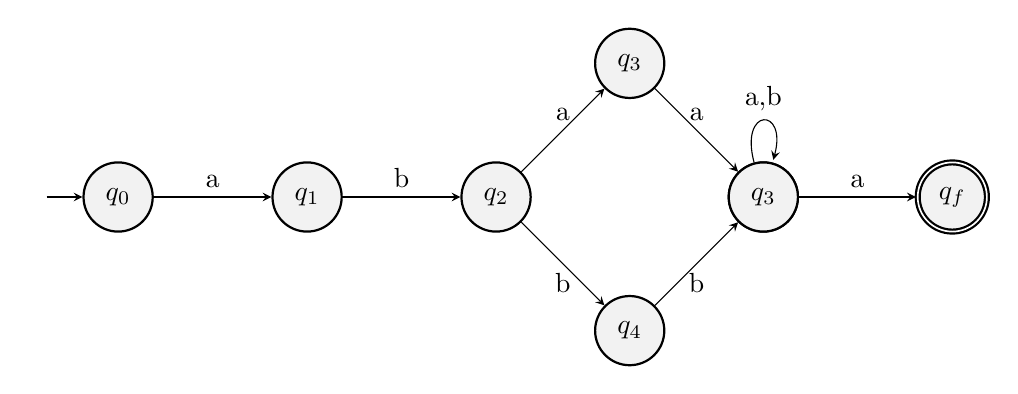
\begin{tikzpicture}
\node[state, initial] (q0) {$q_0$};
\node[state, right of=q0] (q1) {$q_1$};
\node[state, right of=q1] (q2) {$q_2$};
\node[state,above right of=q2] (q3) {$q_3$};
\node[state,  below right of=q2] (q4) {$q_4$};
\node[state, below right of=q3] (q5) {$q_1$};

\node[state,above right of=q4] (q5) {$q_3$};
\node[state, accepting, right of=q5] (qf) {$q_f$};
\draw 

(q0) edge[left,above] node{a } (q1)
(q1) edge[left,above] node{b } (q2)
(q2) edge[right,above] node{a} (q3)
(q2) edge[right,below] node{b} (q4)
(q3) edge[right,above] node{a} (q5)
(q4) edge[right,below] node{b} (q5)
(q5) edge[loop above] node{a,b} (q5)
(q5) edge[right,above] node{a} (qf);


\end{tikzpicture}
%\caption*{Caption.}

\end{figure}

Inserting a new initial state $q_{i}$
 and final state $q_{H}$, the finite automata becomes
 

%-----------------------------------------------------
\begin{figure}[H] % ’ht’ tells LaTeX to place the figure ’here’ or at the top of the page
\centering % centers the figure
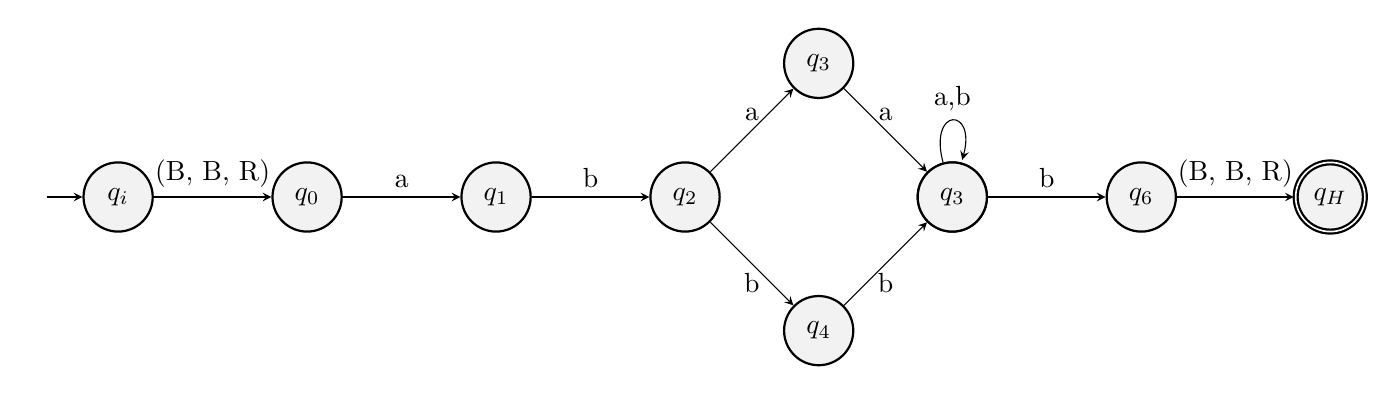
\begin{tikzpicture}
\node[state, initial] (qi) {$q_i$};
\node[state, right of=qi] (q0) {$q_0$};
\node[state, right of=q0] (q1) {$q_1$};
\node[state, right of=q1] (q2) {$q_2$};
\node[state,above right of=q2] (q3) {$q_3$};
\node[state,  below right of=q2] (q4) {$q_4$};
\node[state, below right of=q3] (q5) {$q_1$};

\node[state,above right of=q4] (q5) {$q_3$};
\node[state, right of=q5] (q6) {$q_6$};
\node[state, accepting, right of=q6] (qH) {$q_H$};
\draw 
(qi) edge[left,above] node{(B, B, R) } (q0)
(q0) edge[left,above] node{a } (q1)
(q1) edge[left,above] node{b } (q2)
(q2) edge[right,above] node{a} (q3)
(q2) edge[right,below] node{b} (q4)
(q3) edge[right,above] node{a} (q5)
(q4) edge[right,below] node{b} (q5)
(q5) edge[loop above] node{a,b} (q5)
(q5) edge[right,above] node{b} (q6)
(q6) edge[right,above] node{(B, B, R)} (qH);

\end{tikzpicture}
%\caption*{Caption.}

\end{figure}
Converting the levels of the inputs, the TM becomes

%--------------------------------------------------
\begin{figure}[H] % ’ht’ tells LaTeX to place the figure ’here’ or at the top of the page
\centering % centers the figure
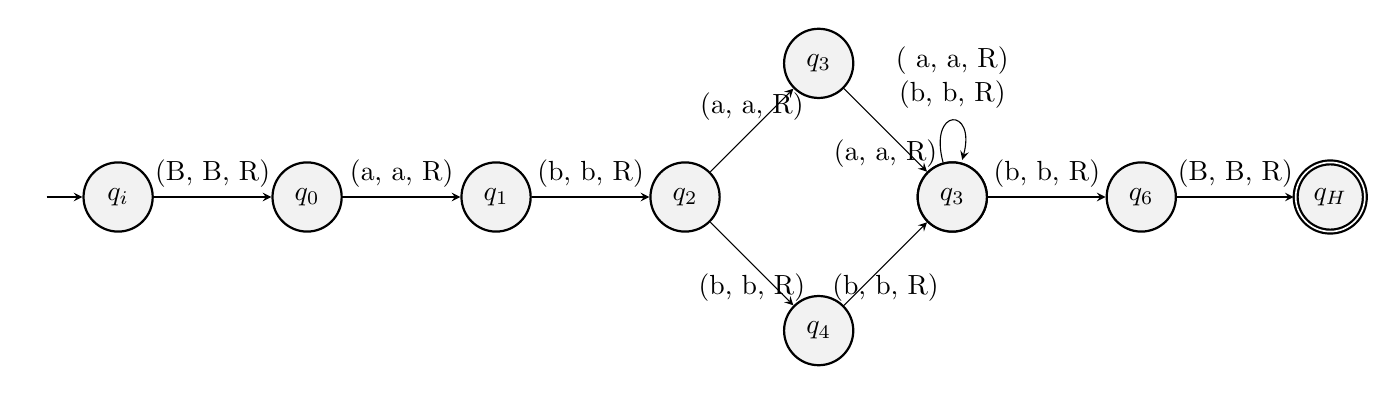
\begin{tikzpicture}
\node[state, initial] (qi) {$q_i$};
\node[state, right of=qi] (q0) {$q_0$};
\node[state, right of=q0] (q1) {$q_1$};
\node[state, right of=q1] (q2) {$q_2$};
\node[state,above right of=q2] (q3) {$q_3$};
\node[state,  below right of=q2] (q4) {$q_4$};
\node[state, below right of=q3] (q5) {$q_1$};

\node[state,above right of=q4] (q5) {$q_3$};
\node[state, right of=q5] (q6) {$q_6$};
\node[state, accepting, right of=q6] (qH) {$q_H$};
\draw 
(qi) edge[left,above] node{(B, B, R) } (q0)
(q0) edge[left,above] node{(a, a, R) } (q1)
(q1) edge[left,above] node{(b, b, R) } (q2)
(q2) edge[right,above] node{(a, a, R)} (q3)
(q2) edge[right,below] node{(b, b, R)} (q4)
(q3) edge[right,below] node{(a, a, R)
} (q5)
(q4) edge[right,below] node{(b, b, R)} (q5)
(q5) edge[loop above] node{\begin{tabular}{c} ( a, a, R) \\ (b, b, R)  \end{tabular}} (q5)
(q5) edge[right,above] node{(b, b, R)} (q6)
(q6) edge[right,above] node{(B, B, R)} (qH);

\end{tikzpicture}
%\caption*{Caption.}

\end{figure}

%-------------------------------------
\begin{figure}[H] % ’ht’ tells LaTeX to place the figure ’here’ or at the top of the page
%\centering % centers the figure
 
\begin{tikzpicture}[every node/.style={single arrow, draw=none, }]

        \node [fill=black,text=white, single arrow head indent=1ex] at (-1.5,0) {Example 8.21};
    \end{tikzpicture}
 Design a TM which converts $(0, 1)_{*}011(0, 1)^{*} to (0, 1)^{*}100(0, 1)^{*}$.

\end{figure}
%----------------------------------------------
\textbf{Solution:} The problem is to design a TM which searches the substring $011$ from a string of $0, 1,$ and then
it replaces 011 by 100. The design is done by the following way.
\begin{enumerate}[i)]
\item  Convert $(0, 1)^{*}011(0, 1)^{*}$ to the accepting DFA.
\item  Convert it to the corresponding TM.
\item  Modify the TM by modifying the transitions of 011 by 100. 
\end{enumerate}

%----------------------------------------------------------
\end{document} 